
\section{Introduction}

A virtual machine provides a ''computer within the computer''. That is, it is a complete \emph{''guest''} computer system with its own hard drive space that can run as an application on a \emph{''host''} computer system. This makes it ideal to deliver a fixed environment with software packages and data sets fully installed and configured. 

A virtual machine is specific to a particular type of computer hardware (processor chip/CPU)and the guest system hardware should be the same as the host system hardware. Hence, when choosing how to proceed, it is important to determine the real computer's hardware. As of this writing, there are two major processor chip/CPU types in use.

\begin{itemize}
\item \emph{Intel and the fully compatible AMD chips} are used primarily with the Windows operating system. However, they were also used by Apple Mac computers until approximately 2021. 
\item \emph{ARM chips} are used in current Apple Mac computers (since approximately 2021, using the Apple M1, M2, or M3 processors/CPU), but are also used in a number of recent Windows laptops (since approximately 2023, using the Qualcomm processors/CPU). 
\end{itemize}

The virtual machine for this course is available for Intel/AMD processors running Windows or MacOS, as well as for ARM processors running MacOS. ARM processors running Windows have not been tested. 

\section{VirtualBox on Windows}

The virtual machine for use on Intel and AMD processors (CPUs) uses the Oracle VirtualBox virtual machine software application. Oracle VirtualBox is free and open-source software that is available at no cost. It comes packaged as a virtual box appliance for import into the VirtualBox software. To install the virtual machine, follow these steps:

\begin{enumerate}
\item Ensure you have approximately 80GB of hard drive space available (30GB to download the virtual box appliance file, and 50GB to install it).
\item Download Oracle VirtualBox from its \href{https://www.virtualbox.org/wiki/Downloads}{website}. Choose the version for your operating system (Windows or MacOS). The virtual machine was developed with VirtualBox version 6.1 but should work with newer versions of VirtualBox. 

\begin{center}
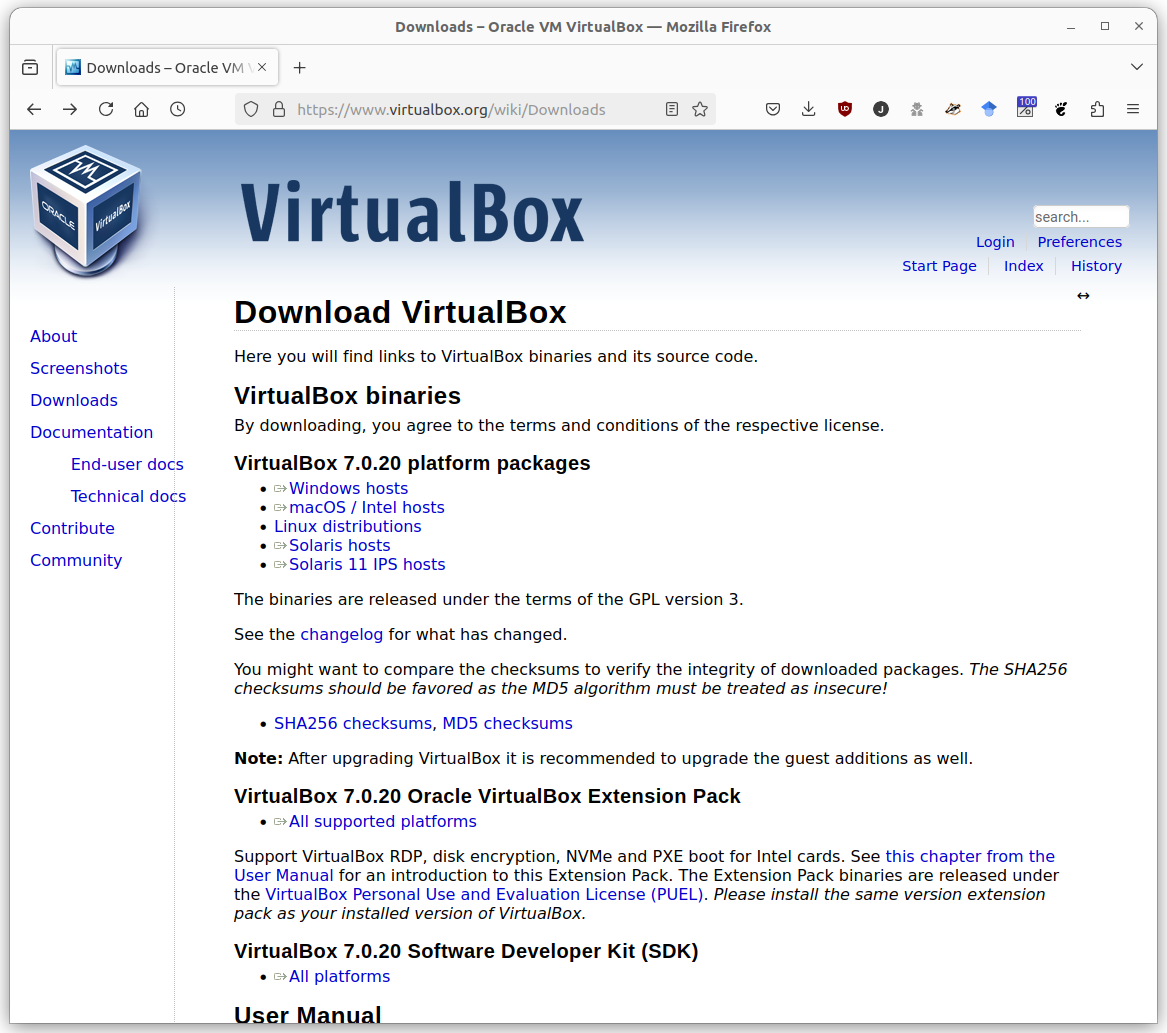
\includegraphics[width=.5\textwidth]{screen2.png}
\end{center}

\item Follow the \href{https://www.virtualbox.org/manual/ch01.html#intro-installing}{general installation instructions} or the \href{https://www.virtualbox.org/manual/ch02.html#installation_windows}{detailed instructions for Windows} or the \href{https://www.virtualbox.org/manual/ch02.html#installation-mac}{detailed instructions for MacOS}. The following screen shots guide you through the installation of VirtualBox on Windows:
   \begin{itemize}
   \item The setup wizard guides you through the setup process. You should confirm default choices:
      \begin{center}
      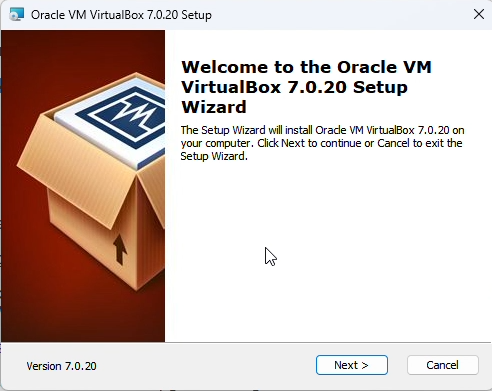
\includegraphics[width=.5\textwidth]{screen4.png}
      \end{center}
   \item Confirm the default features to install:
      \begin{center}
      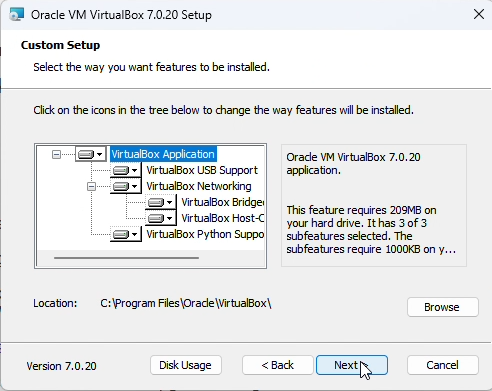
\includegraphics[width=.5\textwidth]{screen5.png}
      \end{center}
   \item Confirm the warning about temporary network disconnect:
      \begin{center}
      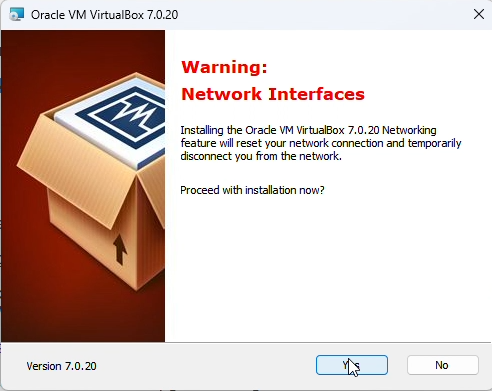
\includegraphics[width=.5\textwidth]{screen6.png}
      \end{center}
   \item Ignore the warning about missing Python dependencies:
      \begin{center}
      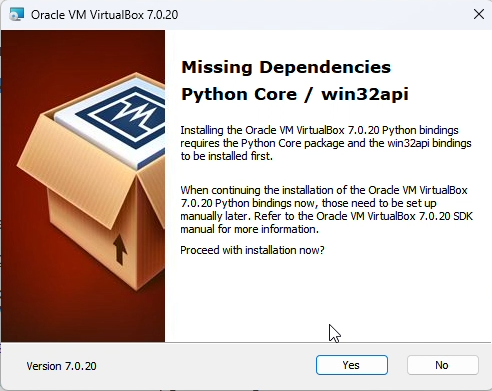
\includegraphics[width=.5\textwidth]{screen7.png}
      \end{center}
   \item Select which menu entries and shortcuts to create according to your preferences:
      \begin{center}
      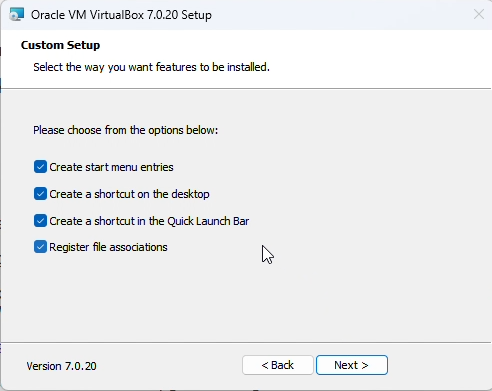
\includegraphics[width=.5\textwidth]{screen8.png}
      \end{center}
   \item Confirm the installation:
      \begin{center}
      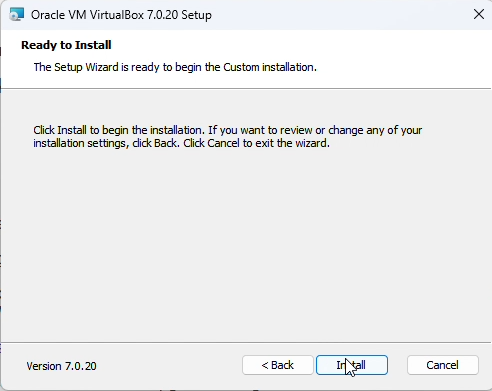
\includegraphics[width=.5\textwidth]{screen9.png}
      \end{center}
   \item Wait for the installation to finish:
      \begin{center}
      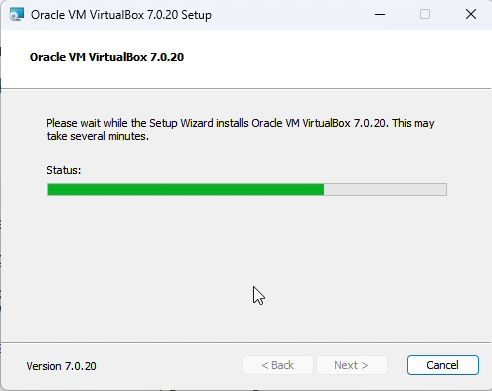
\includegraphics[width=.5\textwidth]{screen10.png}
      \end{center}
   \item Finish the installation, start VirtualBox, and exit the setup wizard:
      \begin{center}
      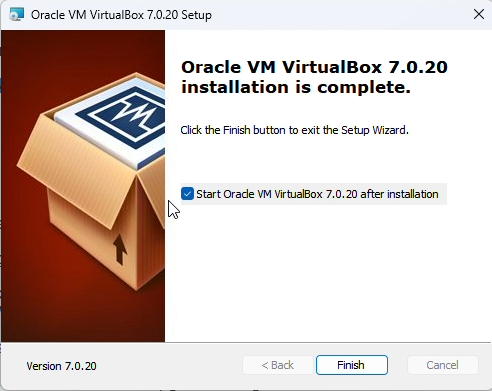
\includegraphics[width=.5\textwidth]{screen11.png}
      \end{center}
   \item You will see the VirtualBox Manager screen:
      \begin{center}
      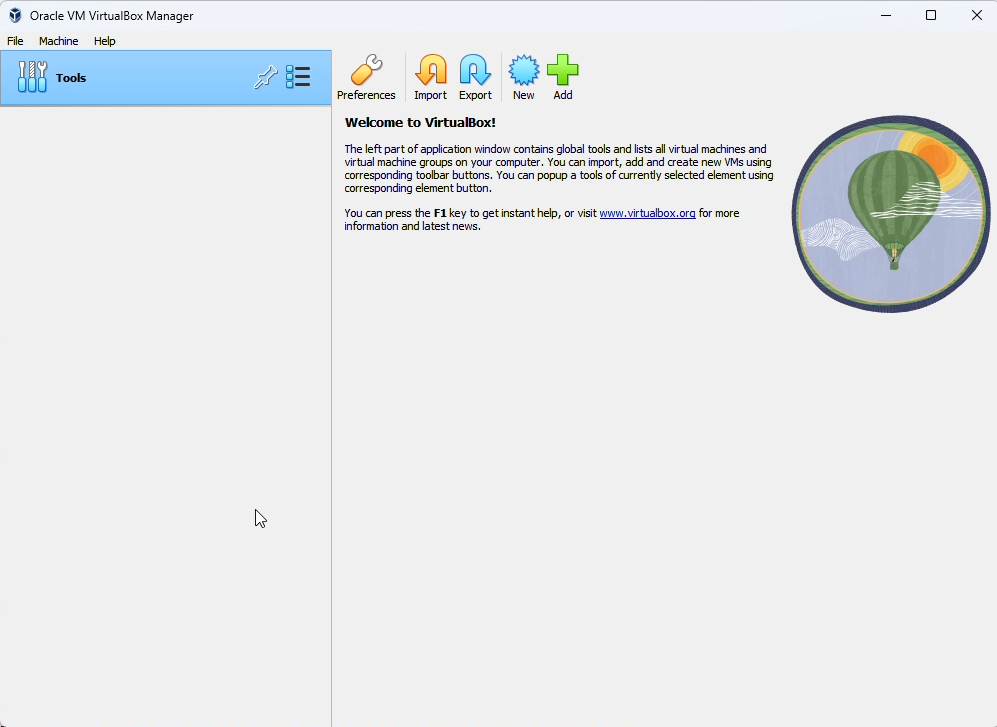
\includegraphics[width=.5\textwidth]{screen12.png}
      \end{center}
   \item Press the ''Preferences'' button. In the general preferences, specify the location for VirtualBox to store the virtual machines. Ensure at least 50GB of hard drive space is avilable in that location:
      \begin{center}
      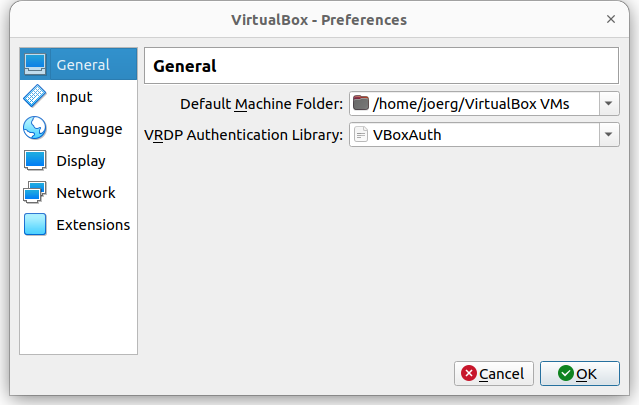
\includegraphics[width=.5\textwidth]{screen1.png}
      \end{center}
\item An overview of the VirtualBox user interface is found in \href{https://www.virtualbox.org/manual/ch01.html}{chapter 1 of the user manual}.
\end{itemize}
\item Download the \href{https://evermann.ca/Busi4720.ova}{virtual appliance file}. \emph{Warning:} This is a 30GB file and will take some time to download.
\item Import the virtual appliance into the VirtualBox software. 
   \begin{itemize}
   \item On the VirtualBox Manager main screen, select ''Import''
      \begin{center}
      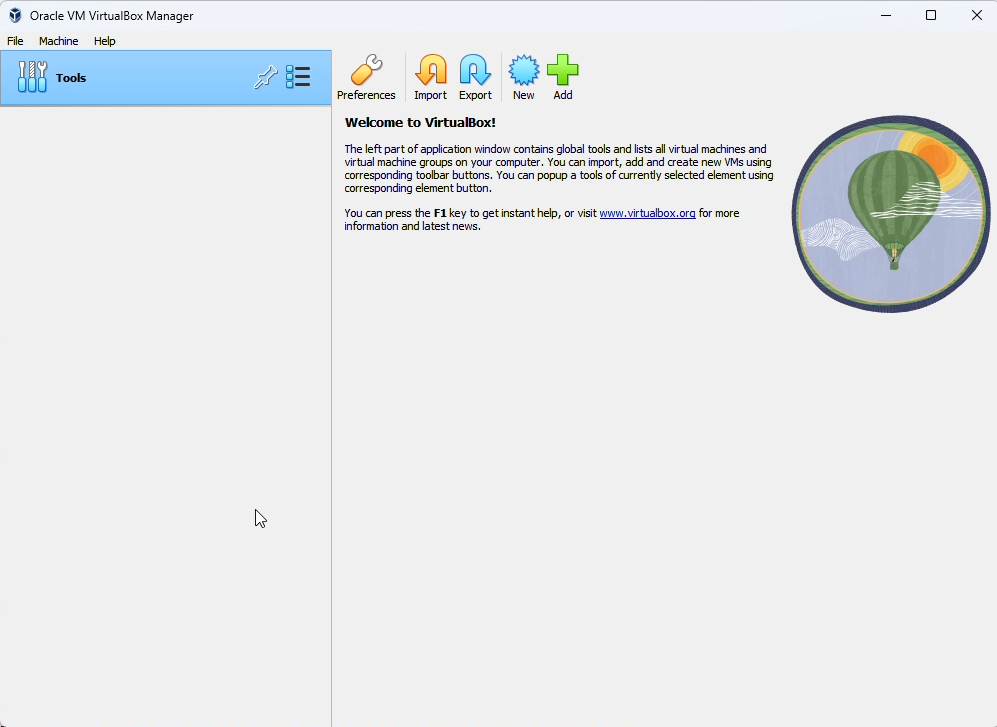
\includegraphics[width=.5\textwidth]{screen12.png}
      \end{center}
   \item Select the virtual appliance file you have downloaded. This is most likely in your ''Downloads'' folder
      \begin{center}
      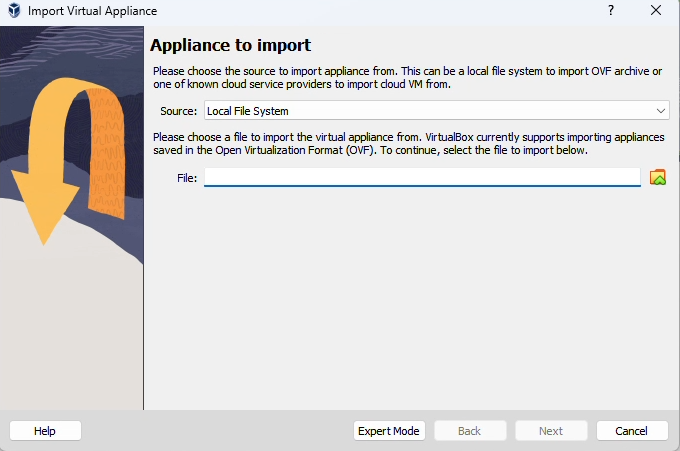
\includegraphics[width=.5\textwidth]{screen13.png}
      \end{center}
      \begin{center}
      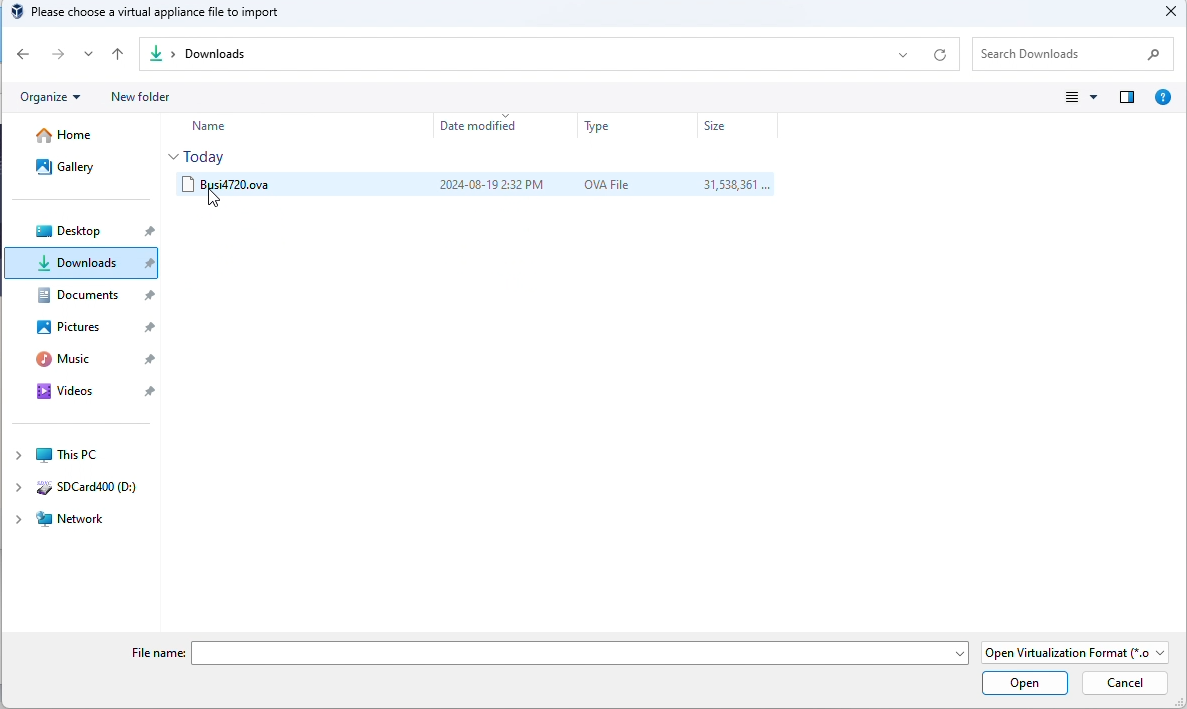
\includegraphics[width=.5\textwidth]{screen14.png}
      \end{center}
      \begin{center}
      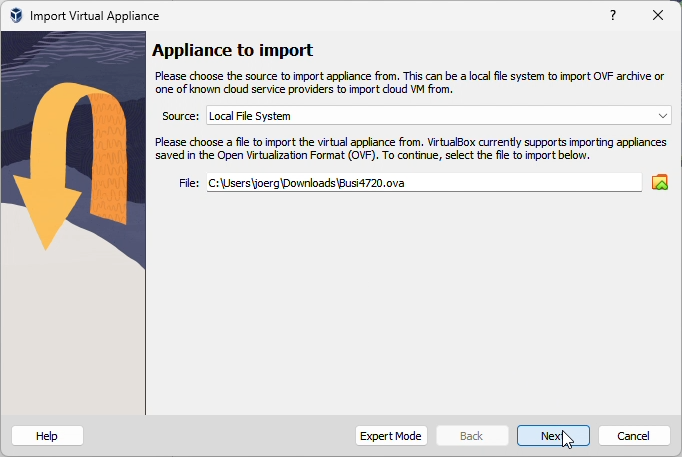
\includegraphics[width=.5\textwidth]{screen15.png}
      \end{center}
   \item Confirm the appliance settings. At this point, you may also choose a different folder than the default one for storing the virtual machine:
      \begin{center}
      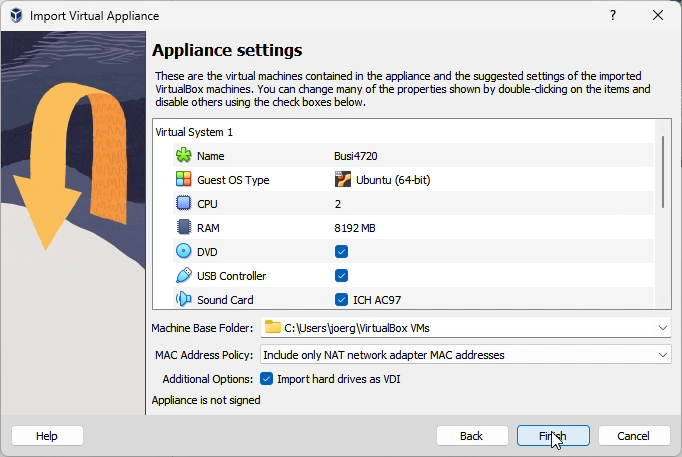
\includegraphics[width=.5\textwidth]{screen16.png}
      \end{center}
   \item Wait for the import to complete. This may take a few minutes.
      \begin{center}
      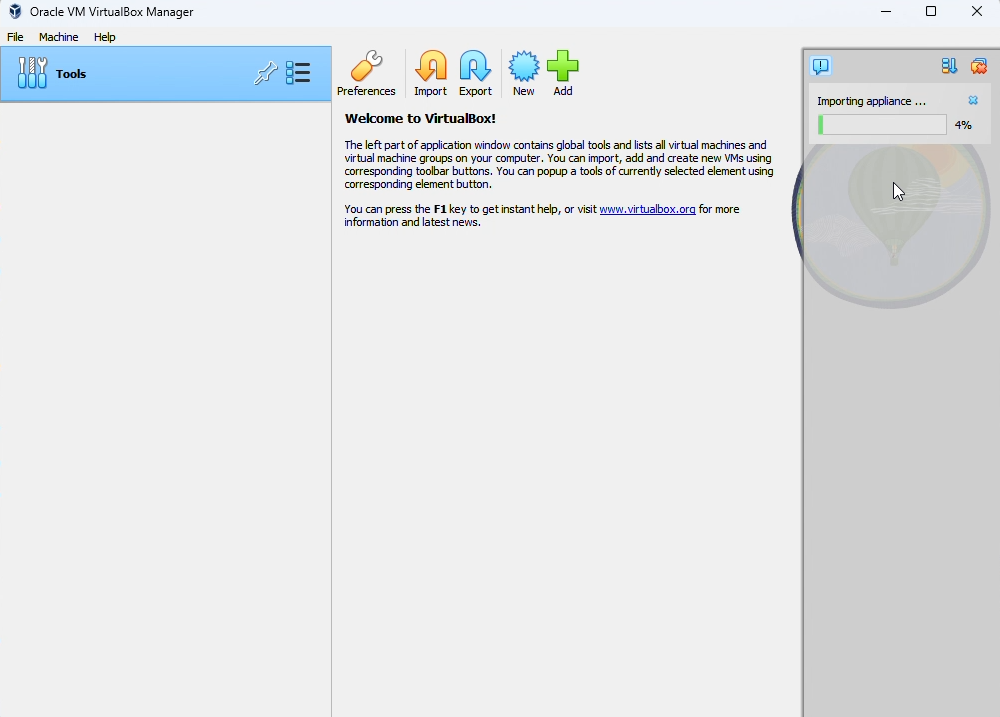
\includegraphics[width=.5\textwidth]{screen17.png}
      \end{center}
   \item When the import is complete, the virtual machine settings will be displayed. Press the ''Settings'' button to change settings for the virtual machine.
      \begin{center}
      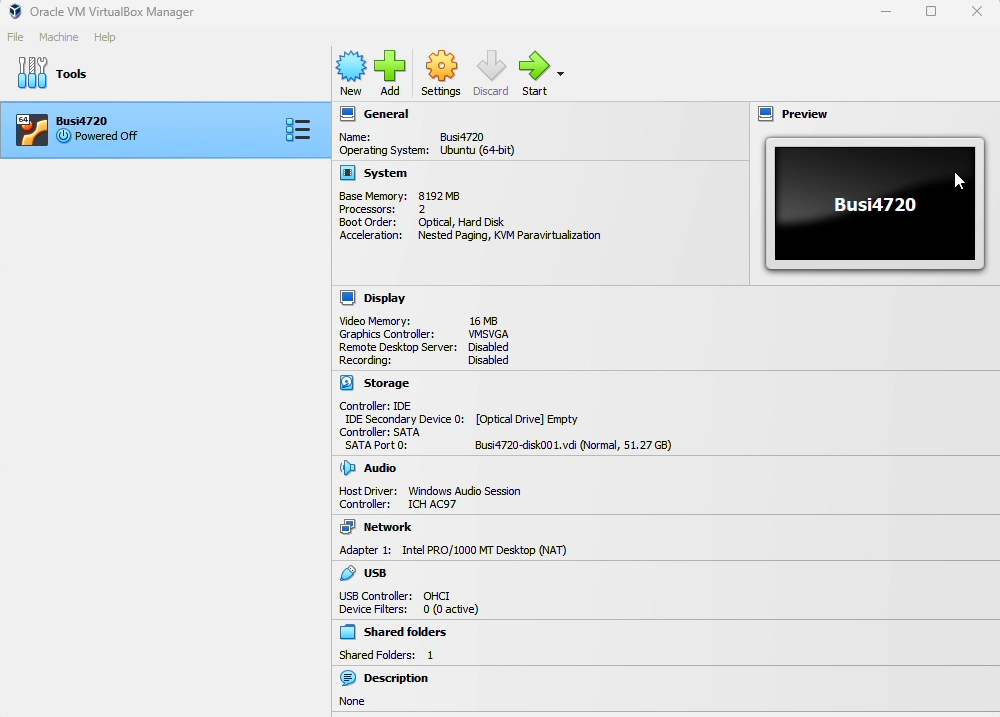
\includegraphics[width=.5\textwidth]{screen18.png}
      \end{center}
   \item In the General settings, you may choose whether to share the clipboard for copy/paste between guest and host, and whether to enable drag-and-drop operations between guest and host.
      \begin{center}
      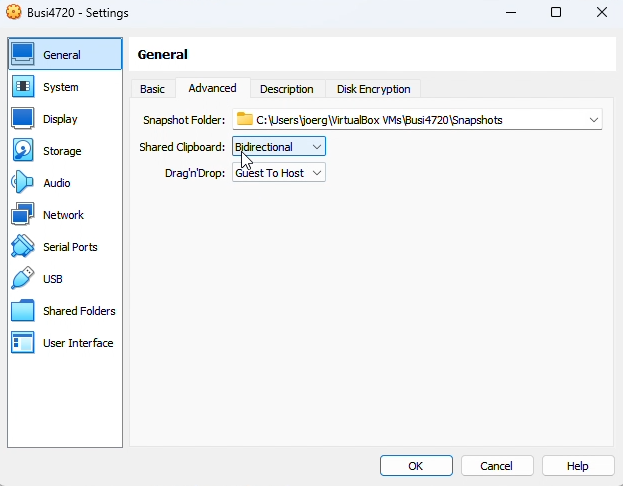
\includegraphics[width=.5\textwidth]{screen19.png}
      \end{center}
   \item In the Systems settings, you may choose how much memory to allocate to the virtual machine. You should allocate around 8000 MB, but ensure that enough memory is left over for the host computer to work smoothly.
      \begin{center}
      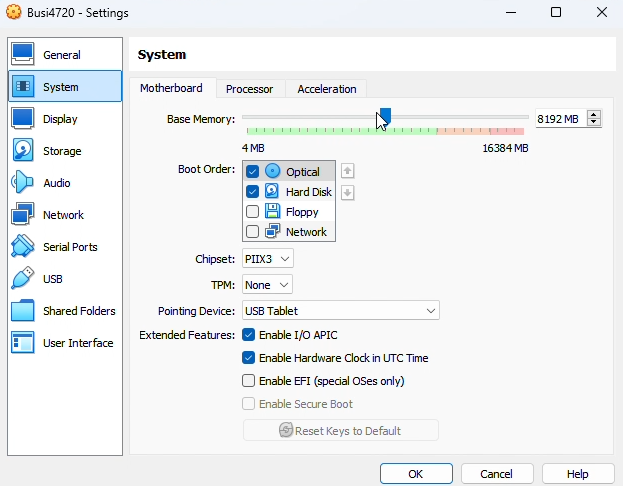
\includegraphics[width=.5\textwidth]{screen20.png}
      \end{center}
   \item In the Processor tab of the Systems settings, you may choose how many processor chips/CPUs to allocate to the virtual machine. Ensure that enough are left over for the host computer to work smoothly.
      \begin{center}
      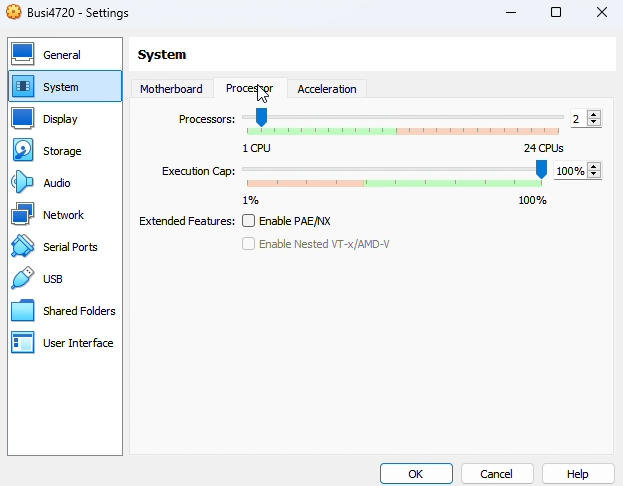
\includegraphics[width=.5\textwidth]{screen21.png}
      \end{center}
   \item In the Display settings, you should allocate all the maximum video memory to the virtual machine. You may also choose a scaling factor. This may be useful if you are working on a very high resolution monitor like an Apple Macbook Retina display.
      \begin{center}
      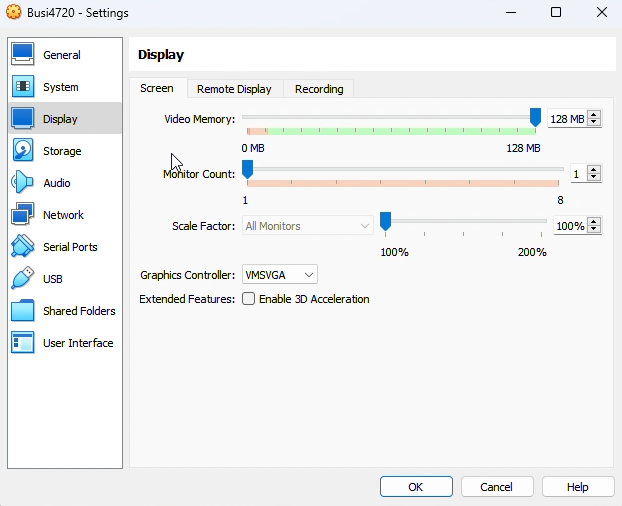
\includegraphics[width=.5\textwidth]{screen22.png}
      \end{center}
   \item In the Shared Folders settings, you should remove any existing shared folders.
      \begin{center}
      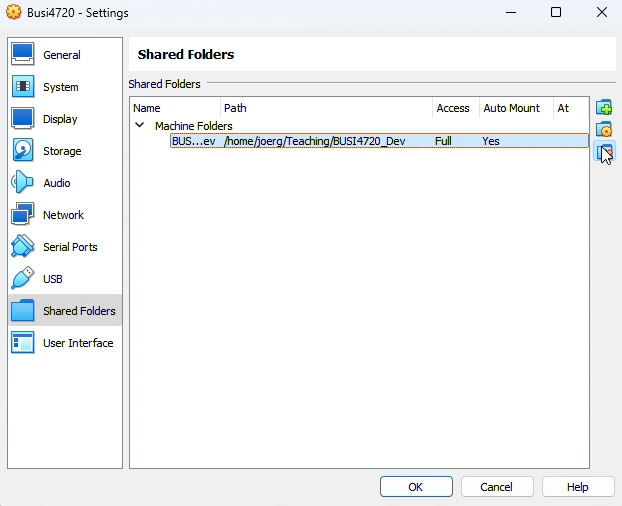
\includegraphics[width=.5\textwidth]{screen23.png}
      \end{center}
   \end{itemize}      
\item Start the virtual machine.
  \begin{itemize}
      \item Press the ''Start'' button on the virtual machine settings overview.
		  \begin{center}
		  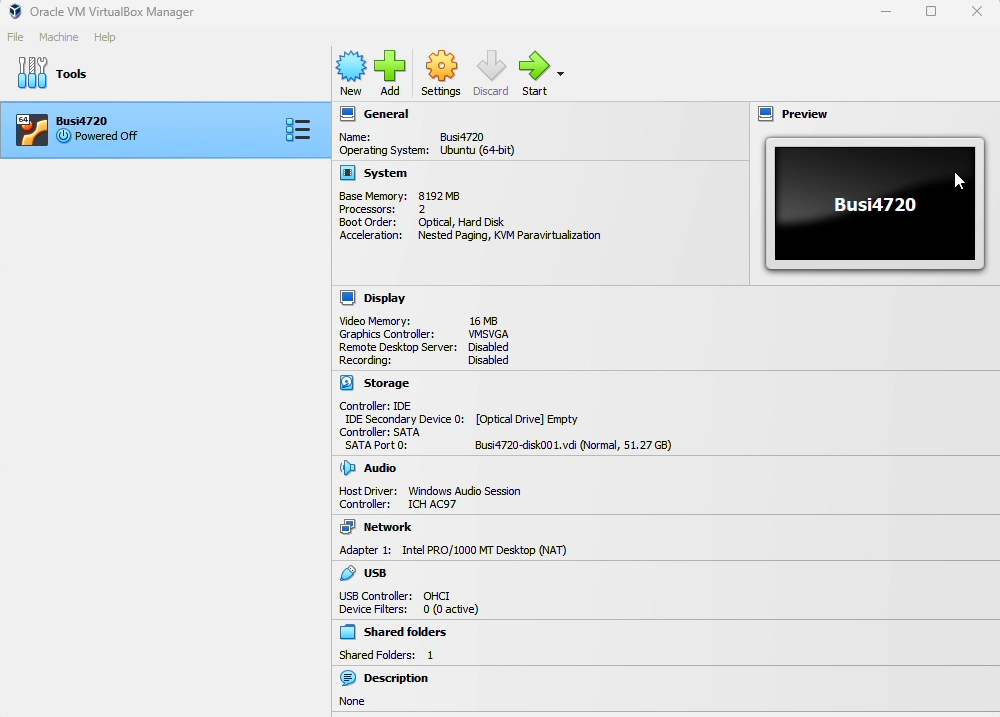
\includegraphics[width=.5\textwidth]{screen18.png}
		  \end{center}
      \item The virtual machine will start and notify you about keyboard and mouse integration. This means your keyboard and mouse inputs will automatically be forwarded from the host to guest system. You can dismiss these messages
		  \begin{center}
		  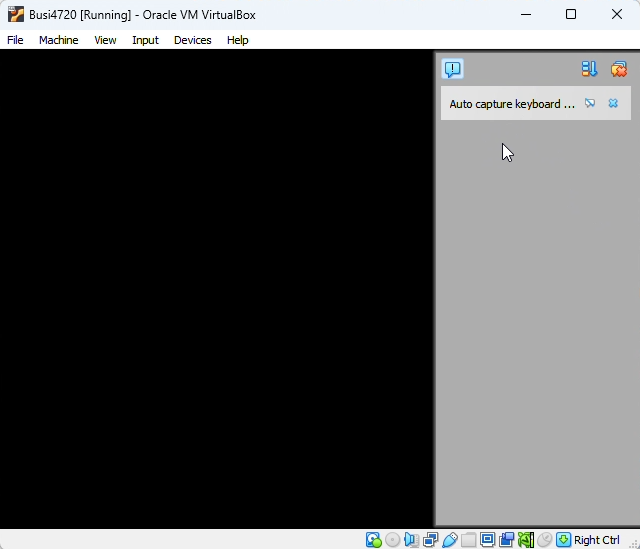
\includegraphics[width=.5\textwidth]{screen24.png}
		  \end{center}
      \item Once the virtual machine has started, you will see the desktop user interface. Popular software applications are accessible via the dock on the left side of the screen. The most important application for working with this book is the Terminal window application.
		  \begin{center}
		  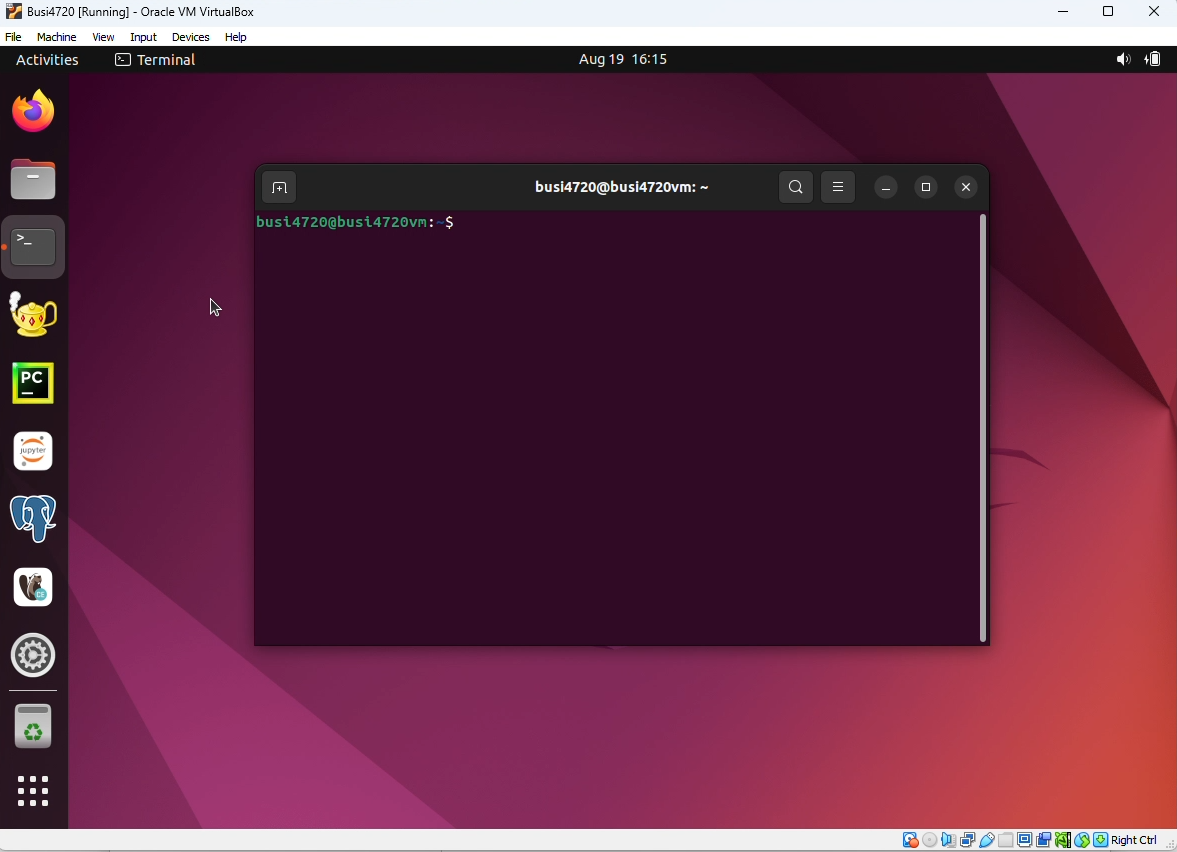
\includegraphics[width=.5\textwidth]{screen26.png}
		  \end{center}
      \item To shut down the virtual machine, select ''Power Off...'' from the system menu in the top right and shut down the machine.
		  \begin{center}
		  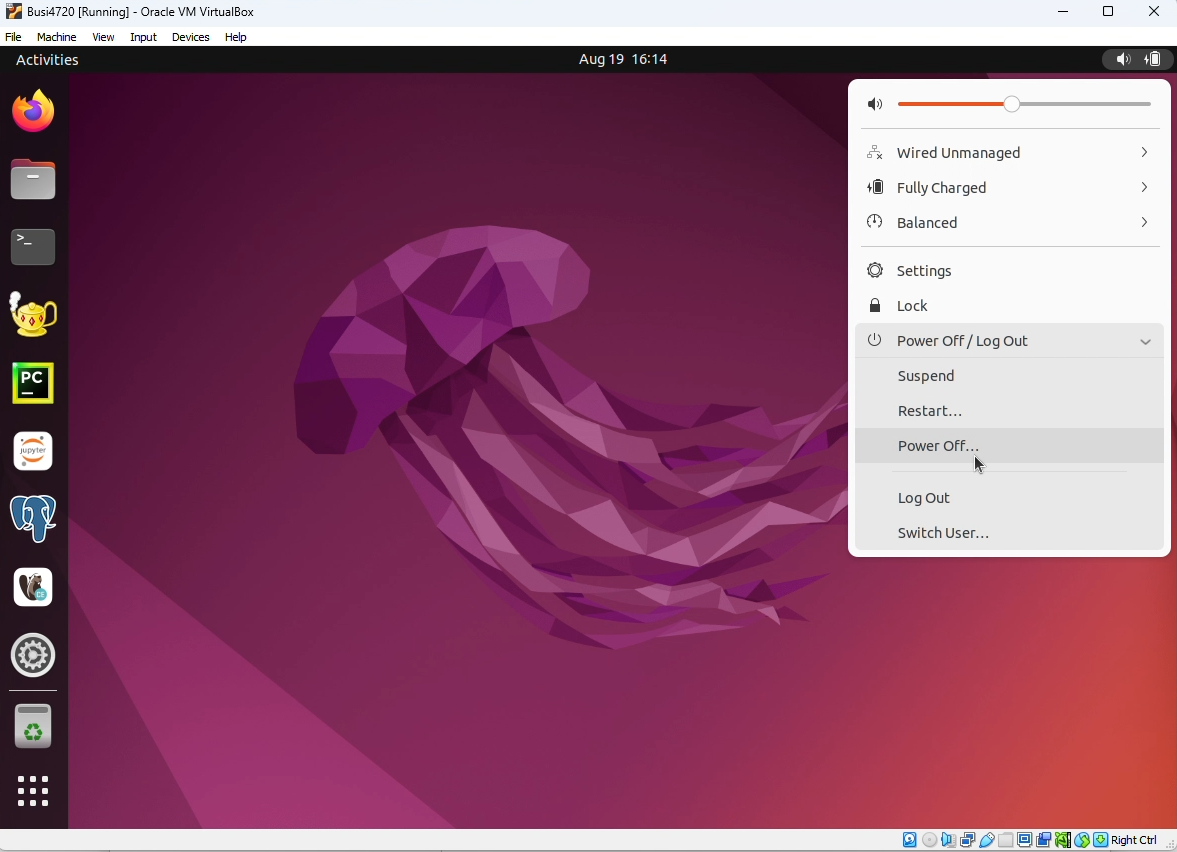
\includegraphics[width=.5\textwidth]{screen25.png}
		  \end{center}
  \end{itemize}
\end{enumerate}


\section{VMWare Fusion on MacOS}
The virtual machine for use on ARM processors (CPUs) uses the VMWare Fusion Pro virtual machine software. VMWare was acquired by Broadcom in 2023. While VMWare Fusion is proprietary software, Broadcom makes it available at no cost for personal use. To install the virtual machine, follow these steps:

\begin{enumerate}
\item Ensure you have approximately 70GB of hard drive space available (20GB to download the virtual machine file, and 50GB to install it).
\item Download VMWare Fusion Pro from its \href{https://support.broadcom.com/group/ecx/productdownloads?subfamily=VMware+Fusion}{website}. You may need to register for a free Broadcom account and login. 
    \begin{itemize}
       \item Choose the latest version of VMWare Fusion Pro for Personal Use. The virtual machine was created with version 13.5.2.
		  \begin{center}
		  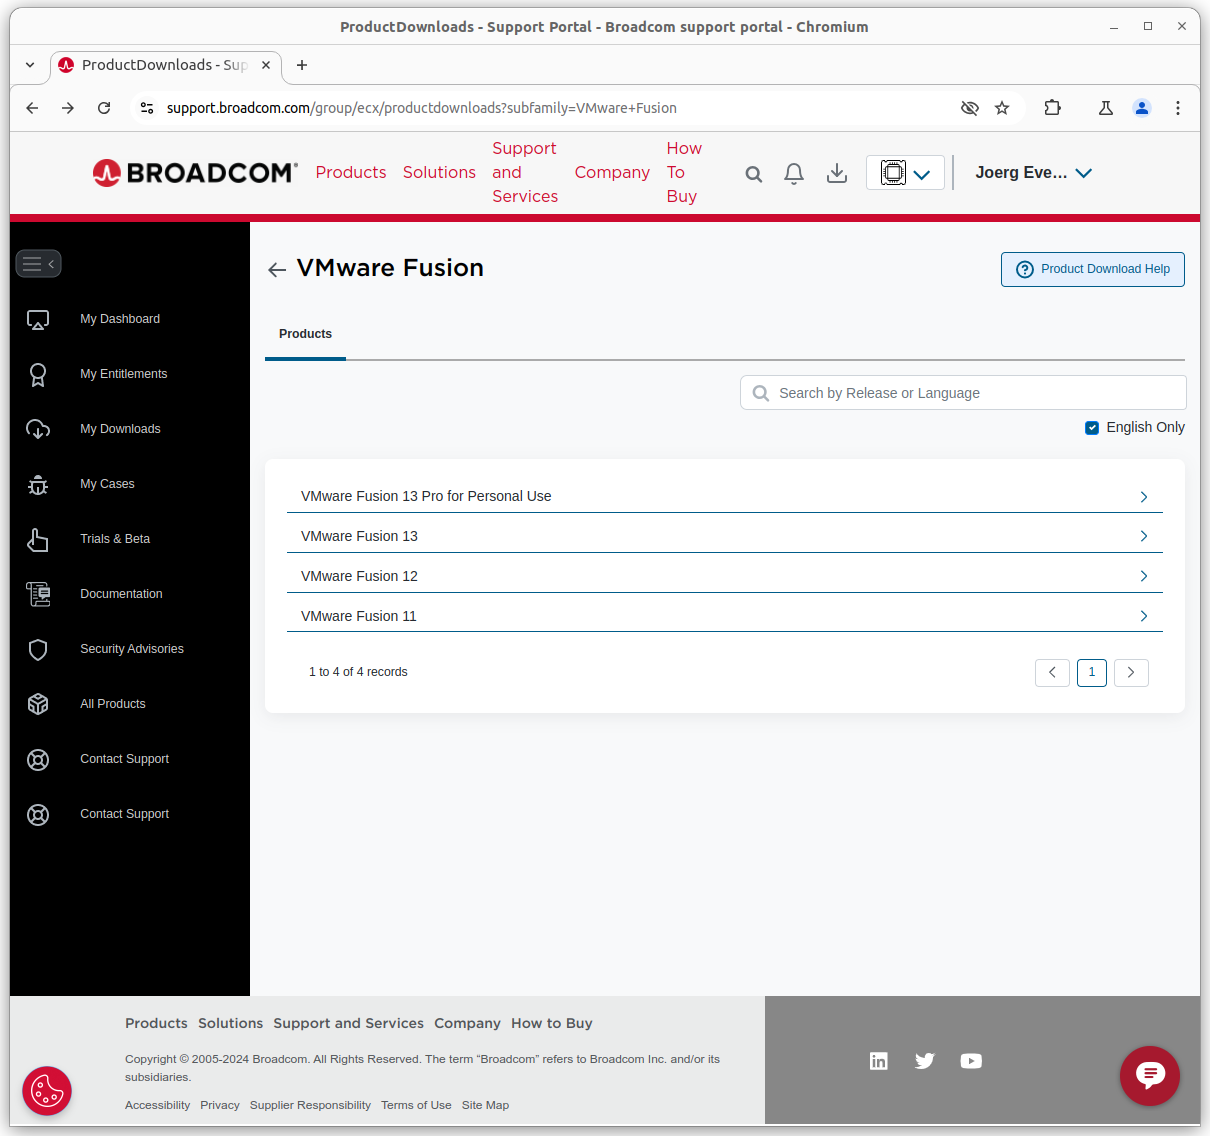
\includegraphics[width=.5\textwidth]{screen28.png}
		  \end{center}
       \item Tick the box to agree to terms and conditions and press the download button next to the VMWare Fusion product.
		  \begin{center}
		  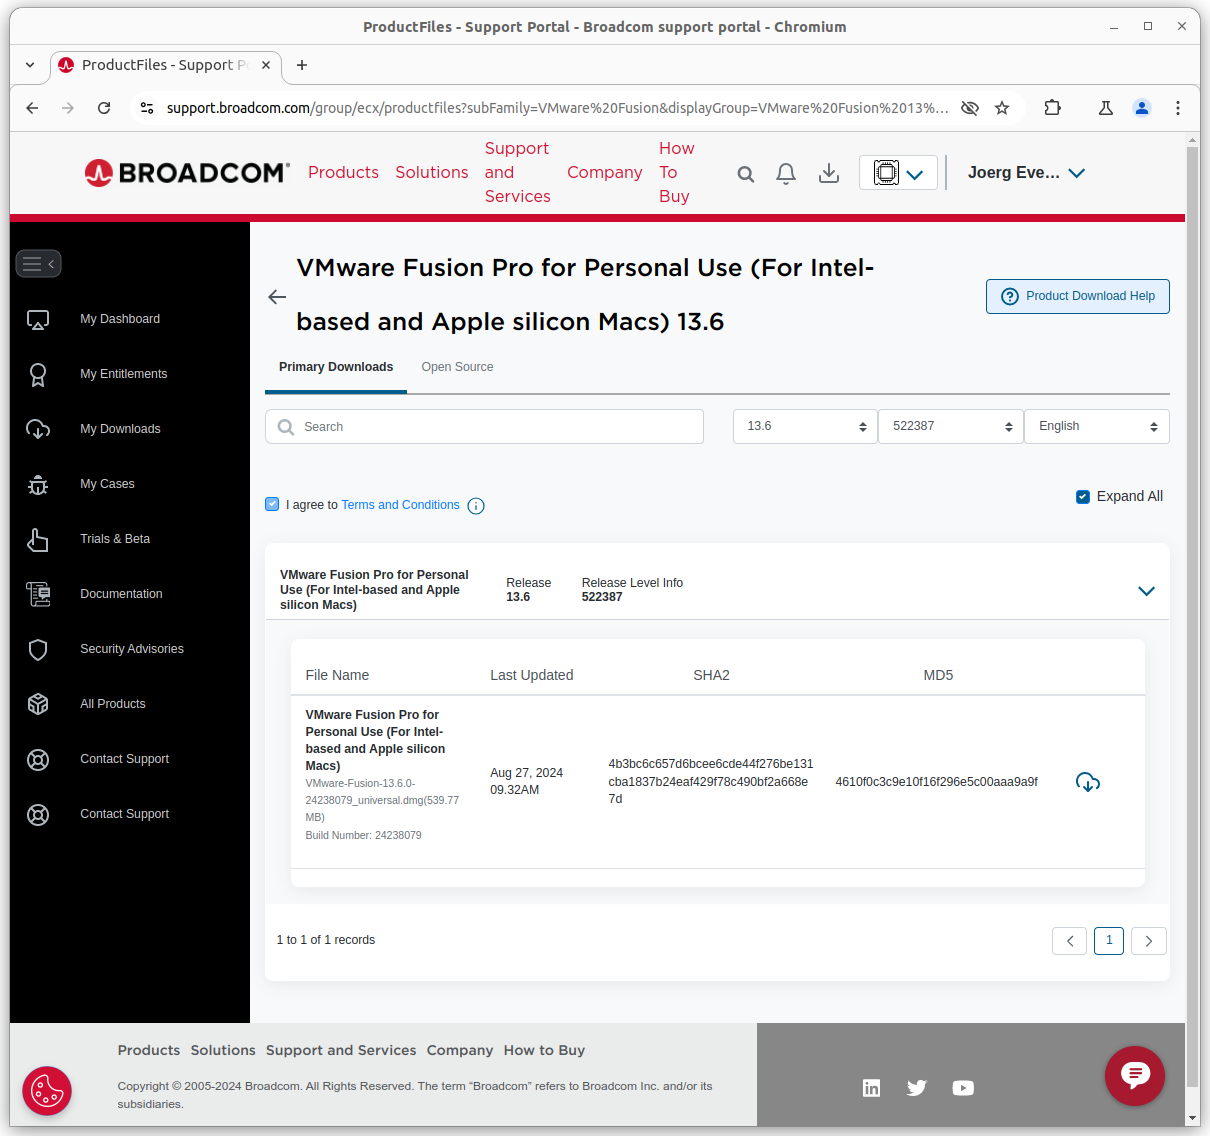
\includegraphics[width=.5\textwidth]{screen27.png}
		  \end{center}
    \end{itemize}
\item Install VMWare Fusion Pro
    \begin{itemize}
       \item Once the download is complete, double-click the downloaded file. You will see the VMware Fusion installer. Double-click it to begin the installation.
		  \begin{center}
		  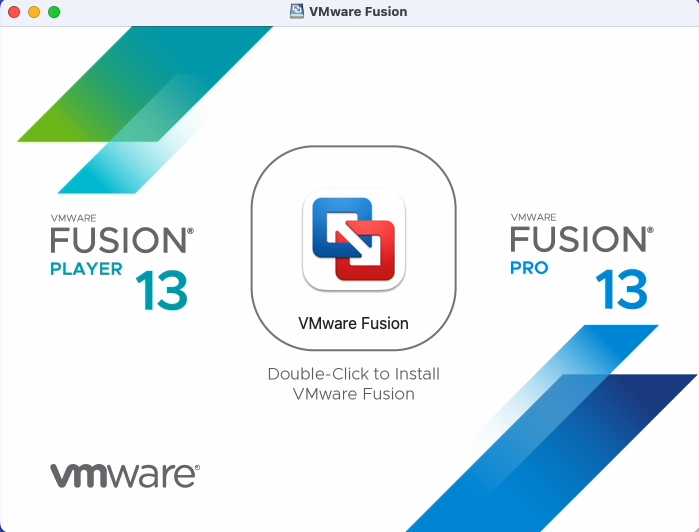
\includegraphics[width=.5\textwidth]{screen29.png}
		  \end{center}
       \item Confirm that you wish to open the application. You may be asked to enter your password to allow this.
		  \begin{center}
		  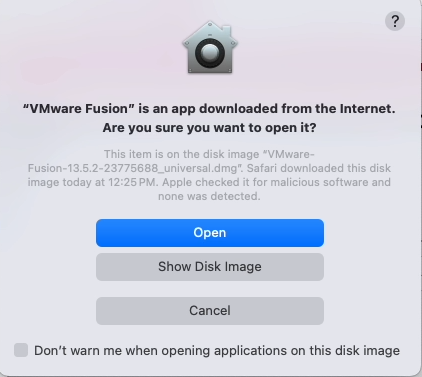
\includegraphics[width=.33\textwidth]{screen30.png}
		  \end{center}
       \item Installation of VMWare Fusion may take a few minutes. 
		  \begin{center}
		  
\includegraphics[width=.33\textwidth]{screen31.png}
		  \end{center}
       \item When installation is complete, VMWare Fusion Pro is launched and will present you with a list of virtual machines or a welcome screen if there are none on your computer.
          \begin{center}
		  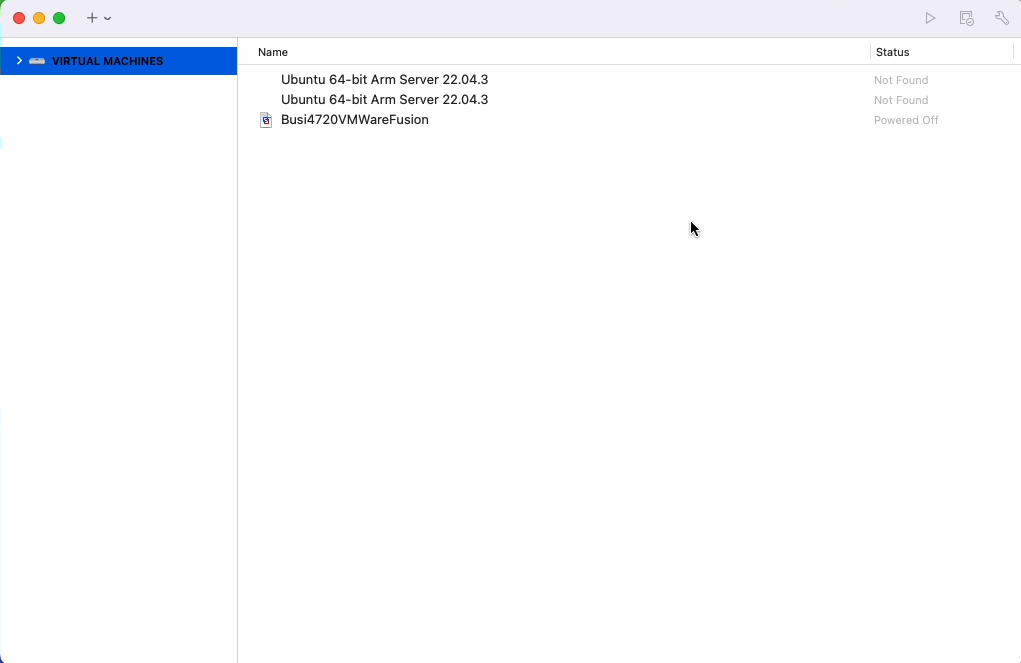
\includegraphics[width=.5\textwidth]{screen32.png}
		  \end{center}
       \item Select ''Settings...'' from the VMWare Fusion main menu bar. 
          \begin{center}
		  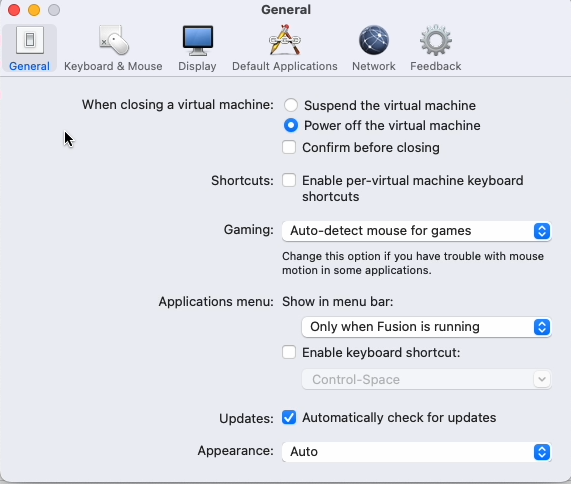
\includegraphics[width=.5\textwidth]{screen33.png}
		  \end{center}
       \item In the Display settings, ensure that resizing the virtual machine is selected both for single window and full screen modes.
          \begin{center}
		  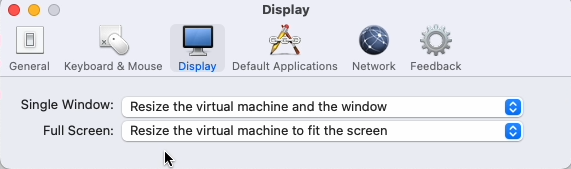
\includegraphics[width=.5\textwidth]{screen34.png}
		  \end{center}
    \end{itemize}
\item Download the \href{https://evermann.ca/Busi4720VMWareFusion.zip}{virtual machine file}. \emph{Warning:} This is a 15GB compressed zip file and will take some time to download. 
    \begin{itemize}
        \item Once the download is complete, the file will be decompressed automatically. This will also take a few minutes of time.
          \begin{center}
		  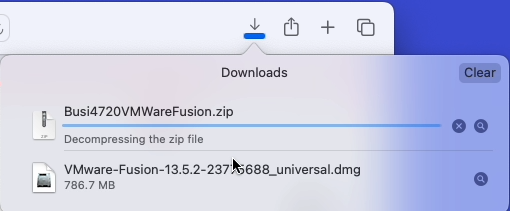
\includegraphics[width=.5\textwidth]{screen35.png}
		  \end{center}
        \item Once the file is downloaded and decompressed, you will be able to see it in your Downloads folder. Expand the ''Busi4720VMWareFusion'' folder to see the uncompressed virtual machine VMBundle.
          \begin{center}
		  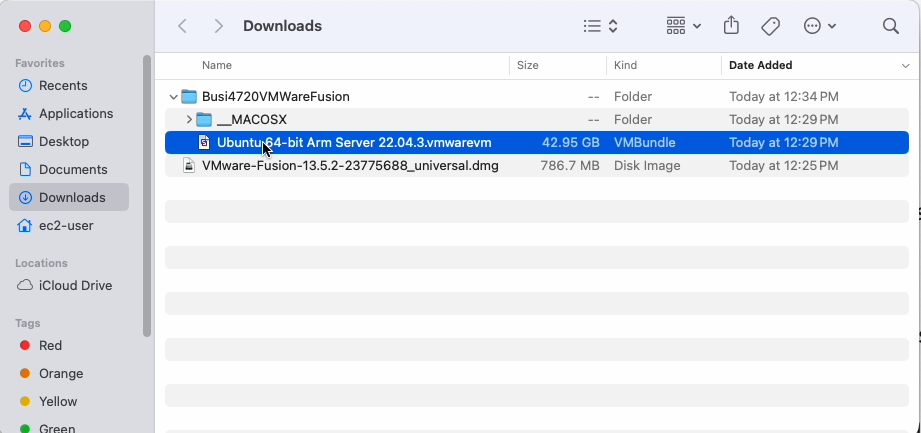
\includegraphics[width=.5\textwidth]{screen36.png}
		  \end{center}
		\item Move this file to a permanent location, for example, to the Documents or Desktop folder.
          \begin{center}
		  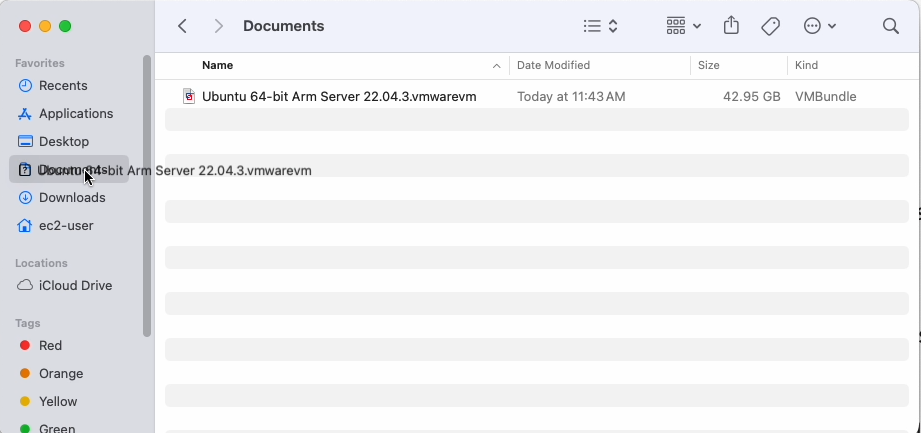
\includegraphics[width=.5\textwidth]{screen37.png}
		  \end{center}
    \end{itemize}
\item Start the virtual machine.
   \begin{itemize}
       \item Double-click on the virtual machine file. This will open the virtual machine in VMWare Fusion Pro.
          \begin{center}
		  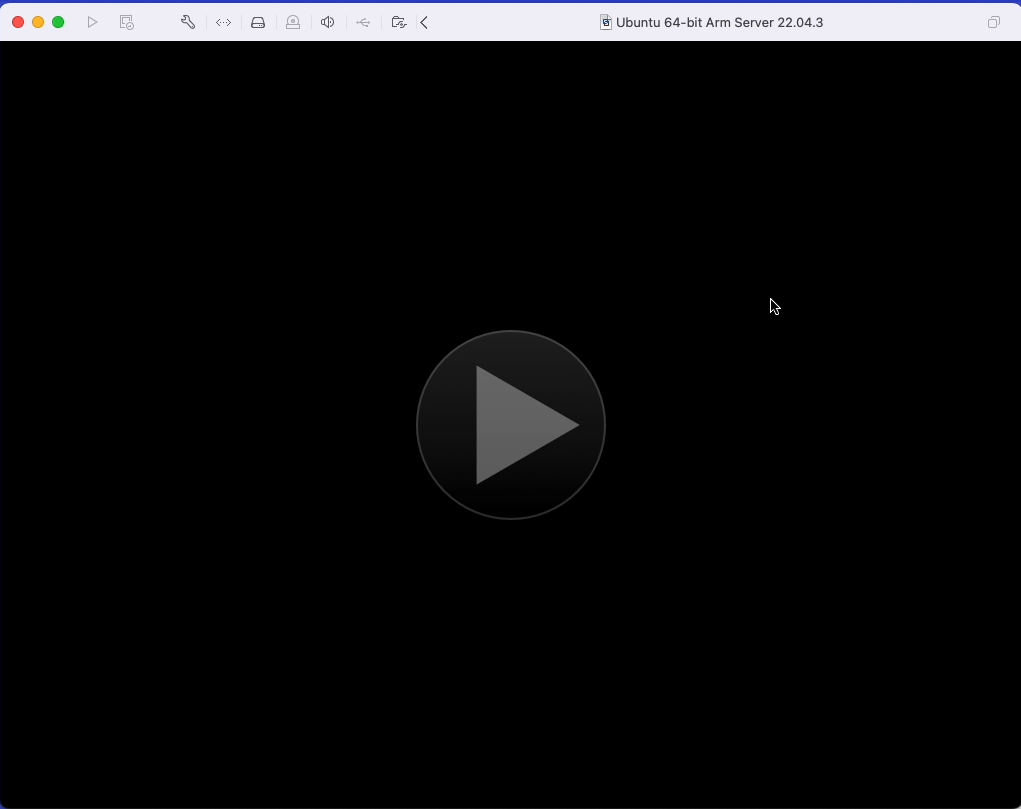
\includegraphics[width=.5\textwidth]{screen38.png}
		  \end{center}
       \item Press the start button to start the virtual machine. The first time you do this, you may be asked whether you copied or moved the machine. Select ''I Copied It''.
          \begin{center}
		  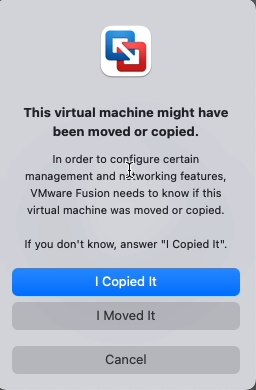
\includegraphics[width=.25\textwidth]{screen39.png}
		  \end{center}
       \item Once the virtual machine has started, you will see the desktop user interface. Popular software applications are accessible via the dock on the left side of the screen. The most important application for working with this book is the Terminal window application.
		  \begin{center}
		  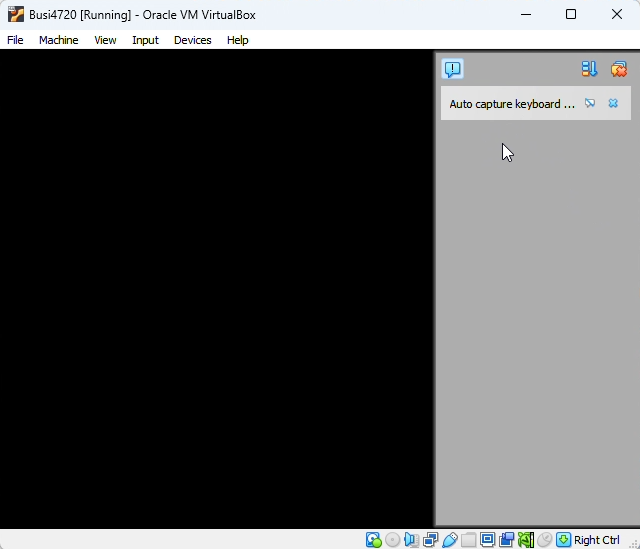
\includegraphics[width=.5\textwidth]{screen24.png}
		  \end{center}
      \item To shut down the virtual machine, select ''Power Off...'' from the system menu in the top right and shut down the machine.
		  \begin{center}
		  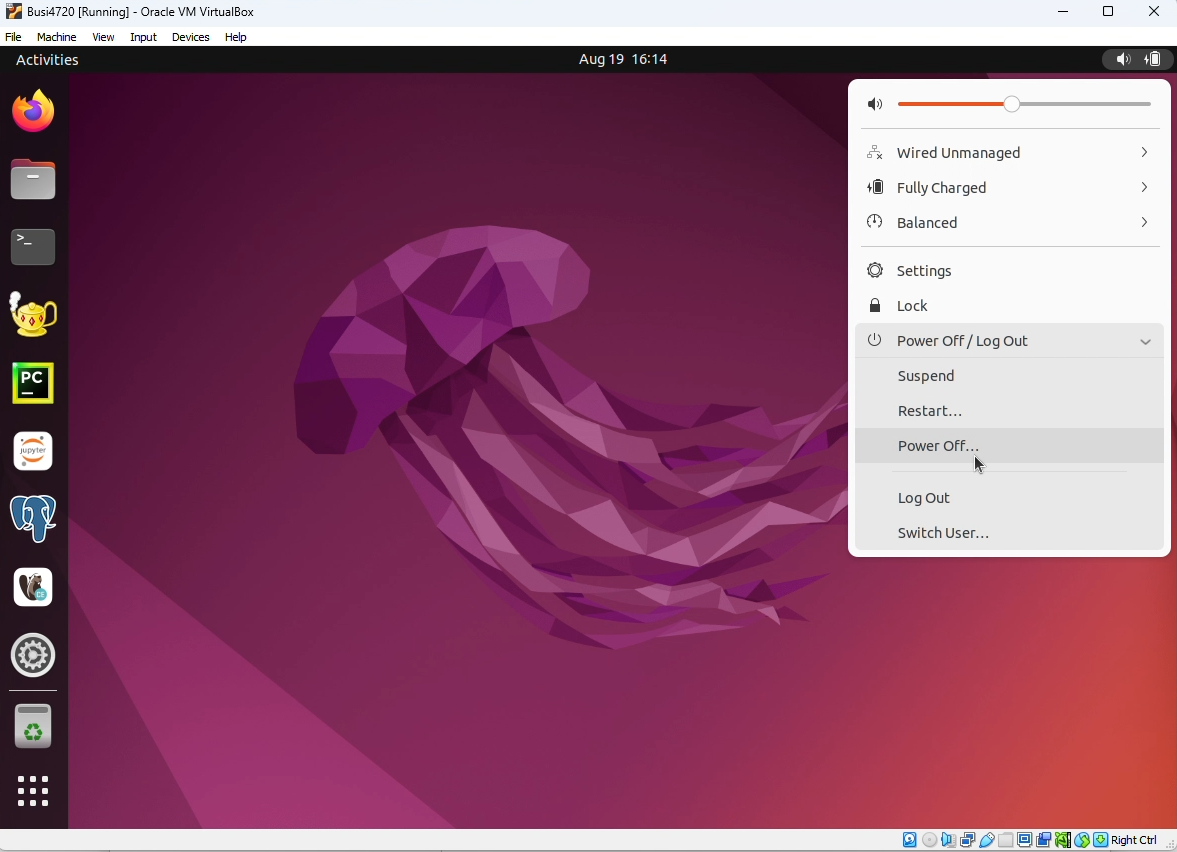
\includegraphics[width=.5\textwidth]{screen25.png}
		  \end{center}
   \end{itemize}
    
\end{enumerate}


